\documentclass[10pt,a4paper]{report}
\usepackage[utf8]{inputenc}
\usepackage{amsmath}
\usepackage{amsfonts}
\usepackage{amssymb}
\usepackage{graphicx}
\usepackage{pgfplots}
\usepackage{pgfplotstable}

\usepackage{fancyhdr}
\usepackage{graphicx}
\usepackage{epstopdf}

\usepackage{hyperref}

\usetikzlibrary{pgfplots.groupplots}

%\usepackage{struktex}
\usepackage{hyperref}
\hypersetup{
    colorlinks=true,
    linkcolor=blue,
    urlcolor=red,
    linktoc=all
}

\graphicspath{{./}}

\usepackage[left=1.5cm,right=1.5cm,top=2cm,bottom=2cm]{geometry}



\definecolor{s1_1}{RGB}{38,70,83}
\definecolor{s1_2}{RGB}{42,157,143}
\definecolor{s1_3}{RGB}{233,196,106}
\definecolor{s1_4}{RGB}{244,162,97}
\definecolor{s1_5}{RGB}{231,111,81}

\definecolor{s2_1}{RGB}{246,81,29}
\definecolor{s2_2}{RGB}{255,180,0}
\definecolor{s2_3}{RGB}{0,166,237}
\definecolor{s2_4}{RGB}{127,184,0}
\definecolor{s2_5}{RGB}{13,44,84}



\pgfplotscreateplotcyclelist{convergelist}{
s2_1, thick, solid, mark=*\\%
s2_2, thick, solid, mark=square\\%
s2_3, thick, solid, mark=diamond*\\%
s2_4, thick, solid, mark=triangle\\%
s2_5, thick, solid, mark=asterisk\\%
}

\pgfplotscreateplotcyclelist{elelist}{
s2_1, solid\\%
s2_2, solid\\%
s2_3, solid\\%
s2_4, solid\\%
s2_5, solid\\%
}




\def \resultspath {../results}
\def \pathpartone {../../1_three-dimensional_atomic_system}
\def \fullpathpartone {/home/lukas/Desktop/project/independence/atomistic_modeling/exam/1_three-dimensional_atomic_system}


\newcommand{\dvec}[1]{\boldsymbol{ \mathsf{#1} } }         % for vectors
\newcommand{\dmat}[1]{\boldsymbol{\mathsf{#1}}}           % for matrices
\newcommand{\Bd}[2]{ (#1,#2)_{D^k} }           % bilienarfor over domian
\newcommand{\Bb}[2]{ (#1,#2)_{\partial D^k} }           % bilienarfor over boundary

\newcommand{\pd}{\partial}
\newcommand{\pdfrac}[2]{\frac{\pd #1}{\pd #2}}  



\title{Report Project 2}
\author{Lukas Scheucher}



\pgfplotstableset{
  col sep=comma,
    create on use/X/.style={create col/copy column from table={/home/lukas/LRZ Sync+Share/Studium/Fach/DG/DG_project/lukas/results/config_task3_K5_N1_LF_x.dat}{0}}
}



\begin{document}


\chapter{Three-dimensional atomistic system}
For the determination of the lattice constant and lattice type, 3 different configurations are considered:
\begin{enumerate}
\item Face-centered cubic (FCC)
\item Body-centered cubic (BCC)
\item Primitive cubic     (PC)
\end{enumerate}
The system will take those configuration, which shows the least total energy per atom. Since interactions happen not only with the closes neighbors, but also with other atoms, an simulation has to be performed to get the exact energys.\\
However, a good first approximation can be made analytically by considering the following observations: All atoms within a lattice type are equal, meaning that an atom that appears as a center atom in BCC can also be viewed as a corner atom just by shifting the connections. Secondly, if one denoted the length of the cube as lattice constant $a$, one can easily determine the distances between all atom by simple geometric means.\\
By looking only at the closest neighbours, one can derive the following expression for the energy per atom in all 3 grids:
\begin{align}
E_{FCC}&=6 U(a_{FCC})+12 U(a_{FCC}/\sqrt{2}) \\
E_{BCC}&=6 U(a_{BCC})+8 U(a_{BCC} \sqrt{3}/2) \\
E_{PC} &=6 U(a_{PC})
\end{align}

By solving for local minima, the following lattice constants are obtained
\begin{align}
a_{FCC,min}&= 5.7432\AA\\
a_{BCC,min}&= 4.6143\AA\\
a_{PC,min} &= 4.097\AA\\
\end{align}

Susbstitutin this back in to the equation for the energies per atom, one can see, that the FCC configuration with an approximate lattice constant of $5.7432\AA$ gives the smalles total energy and is therfore the configuration obtained.\\

Scripts used for this question:
\href{../../lattice_constant_approximation.m}{lattice\_constant\_approximation.m}


Of course, the lattice constant can also be obtained by simulations. This has been done with the input script \href{../../DIR1/in.latticeconstant}{in.latticeconstant}. To run the simulations just call \href{../../DIR1/run_latticeconstant.sh}{run\_latticeconstant.sh}.\\
The lattice-constant obtained after minimization is $5.64 \AA$. The minimization process is visualized in Figure~\ref{fig:p1_latticeconst}.

\begin{center}
\begin{figure}[h]
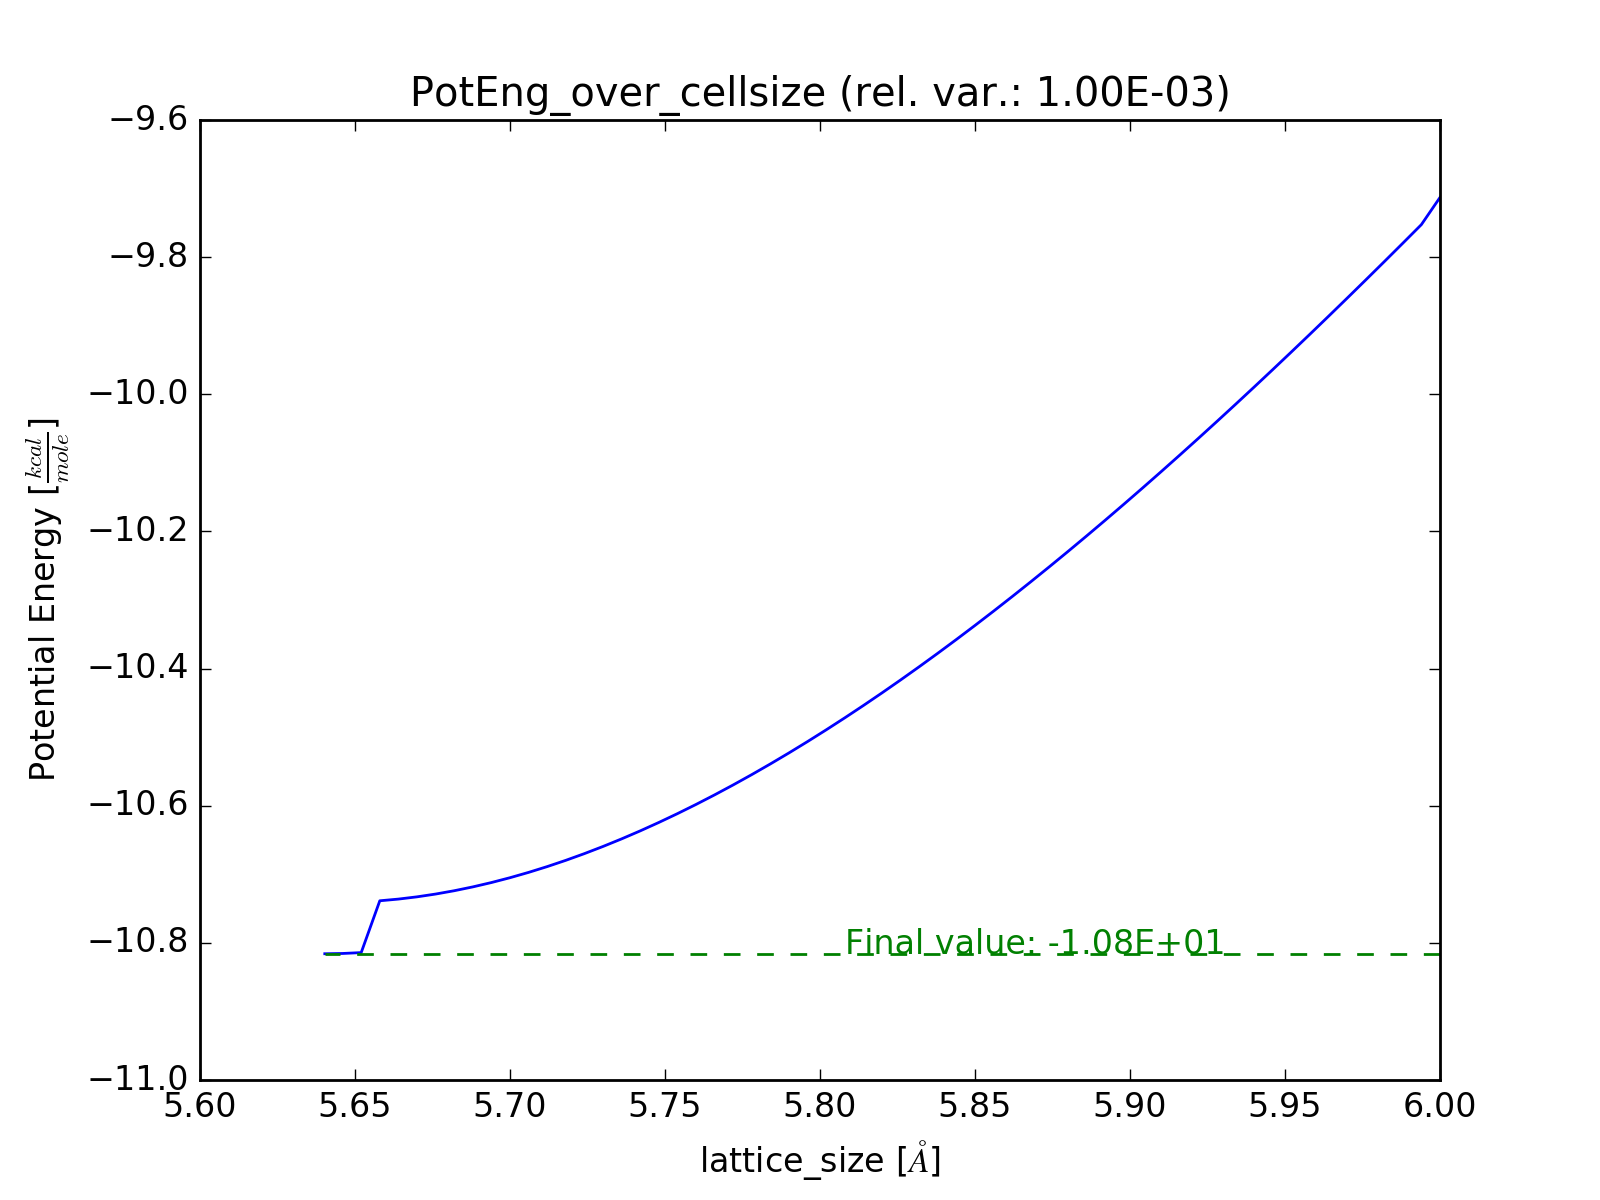
\includegraphics[width=0.5\textwidth]{\fullpathpartone/plots/latticeconst/PotEng_over_Lx.png}~
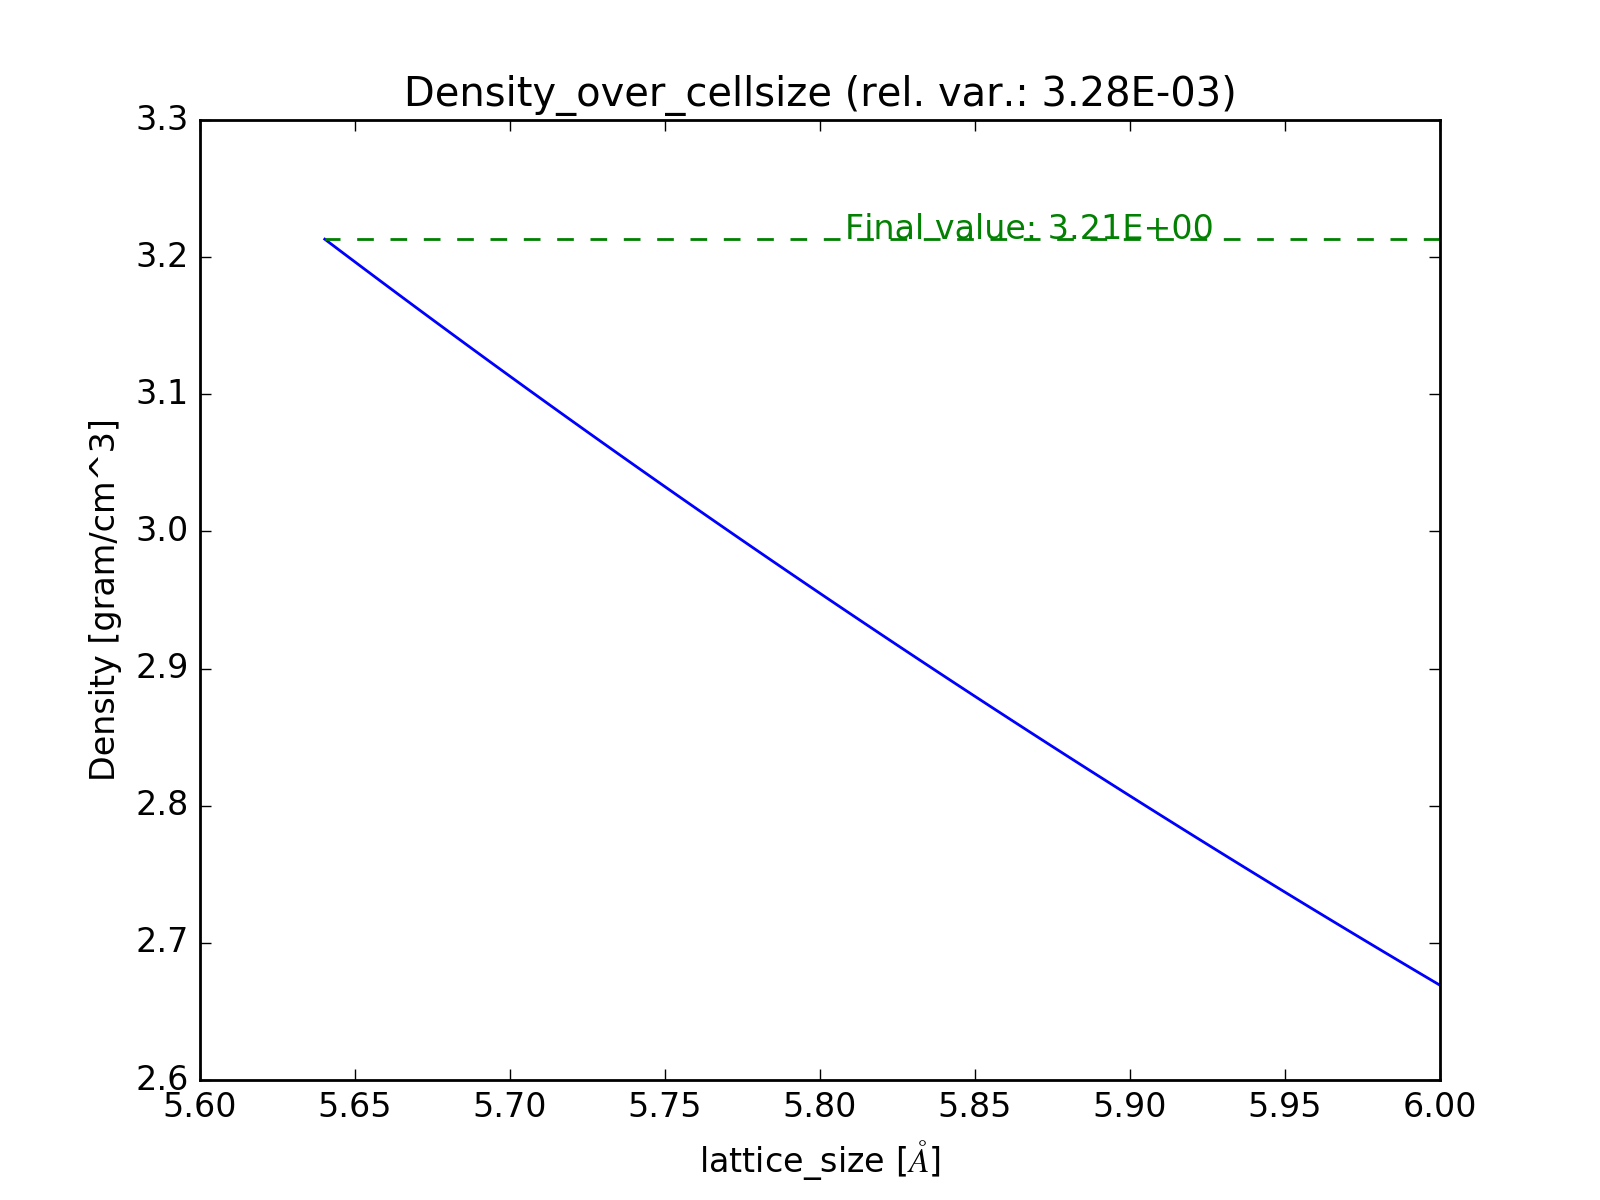
\includegraphics[width=0.5\textwidth]{\fullpathpartone/plots/latticeconst/Density_over_Lx.png}~
\caption[aa]{Convergence of Potential energy on the left, Final density value on the right. The final lattice-constant determined by the simulation is \textbf{5.640 $\AA$}. }
\label{fig:p1_latticeconst}
\end{figure}
\end{center}


\section{Constant temperature and molecular dynamics}
Through several simulations, a timestep of $10 fs$ has been determined as stable. The inputfiles for all simulations are \href{\pathpartone/in.NVT_template}{in.NVT\_template} for the Noose-Hover thermostat and \href{\pathpartone/in.NVEBer_template}{in.NVEBer\_template} for the "weak-coupling" Berendsen thermostat.

\subsection{Equilibriation}
For the equilibriation phase, the lattice constant of $5.90 \AA$, as states on the instruction, has been used. The results are plotted in Figure~\ref{fig:p1_equilibriation}. All relative variances have been calculated after the system has reached equilibrium. The plots show, that the weakly coupled Berendsen thermostat capable of delivering the exact temperature value. However, while damping helps to reduce the fluctuation in Potential energy, it increases the variance of the temperature values. For the NVT thermostat on the other hand, damping can help to reduce fluctuations in all quantities of interest.\\
Overall, the weakly-coupled Berendsen thermostat clearly performs superior compared to Nose-Hoover.

\begin{center}
\begin{figure}[h]
g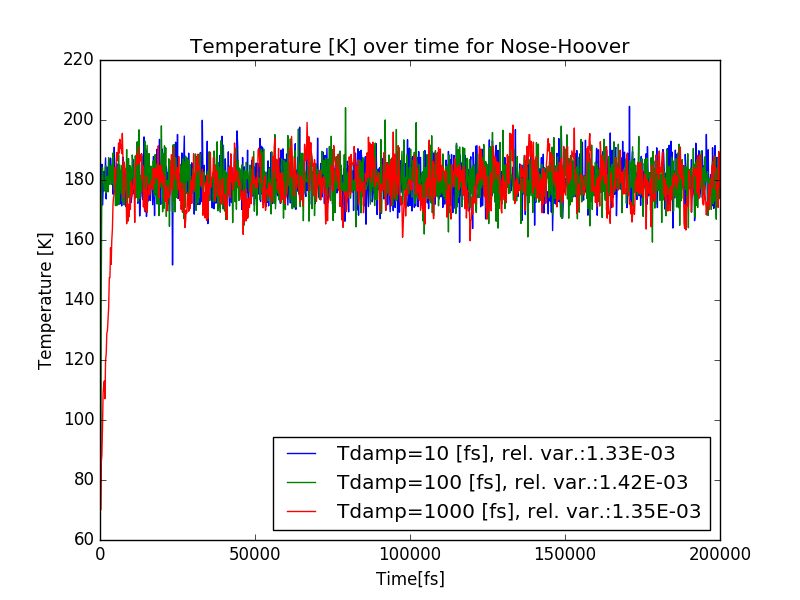
\includegraphics[width=0.5\textwidth]{\fullpathpartone/plots/dampstudy/NVT_Temp_atomnum500.png}~
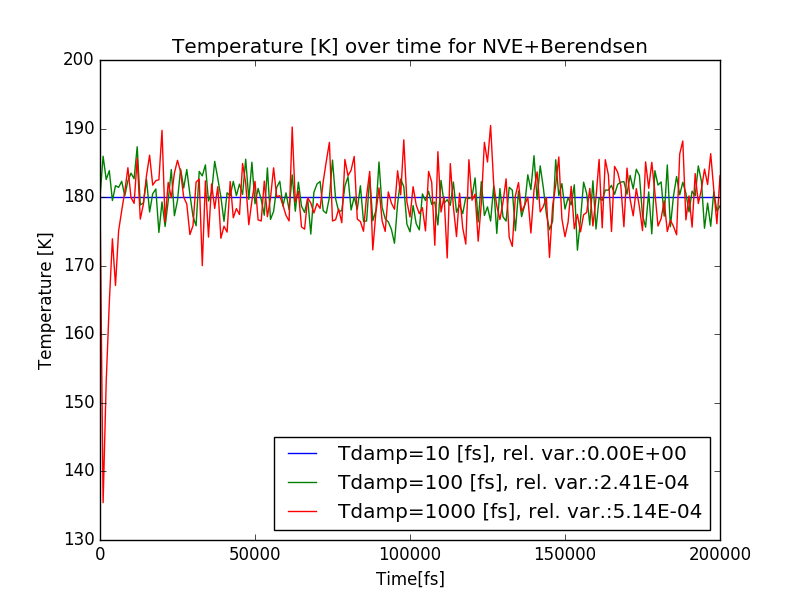
\includegraphics[width=0.5\textwidth]{\fullpathpartone/plots/dampstudy/NVEBer_Temp_atomnum500.png}
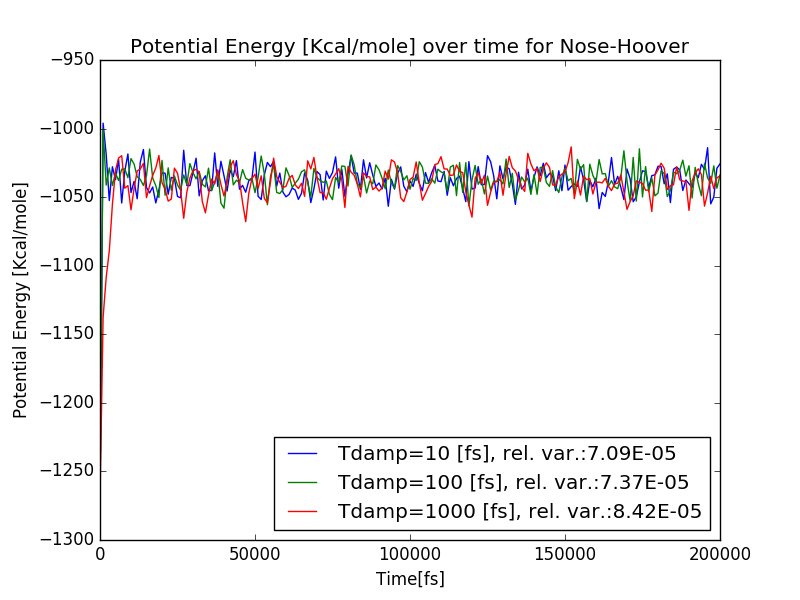
\includegraphics[width=0.5\textwidth]{\fullpathpartone/plots/dampstudy/NVT_PotEng_atomnum500.png}~
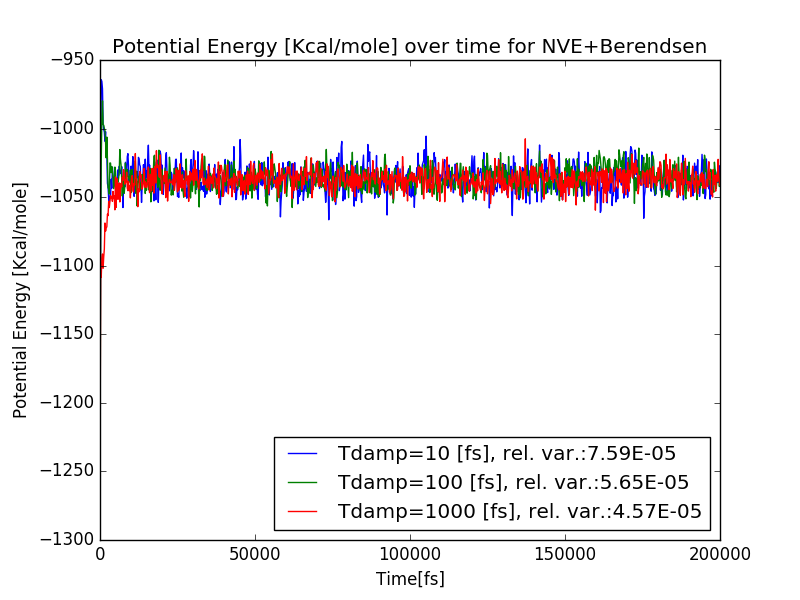
\includegraphics[width=0.5\textwidth]{\fullpathpartone/plots/dampstudy/NVEBer_PotEng_atomnum500.png}
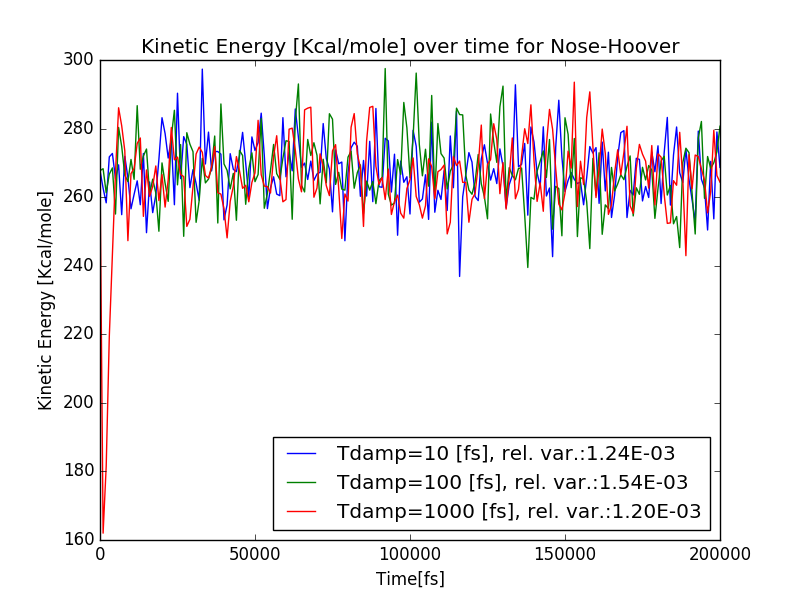
\includegraphics[width=0.5\textwidth]{\fullpathpartone/plots/dampstudy/NVT_KinEng_atomnum500.png}~
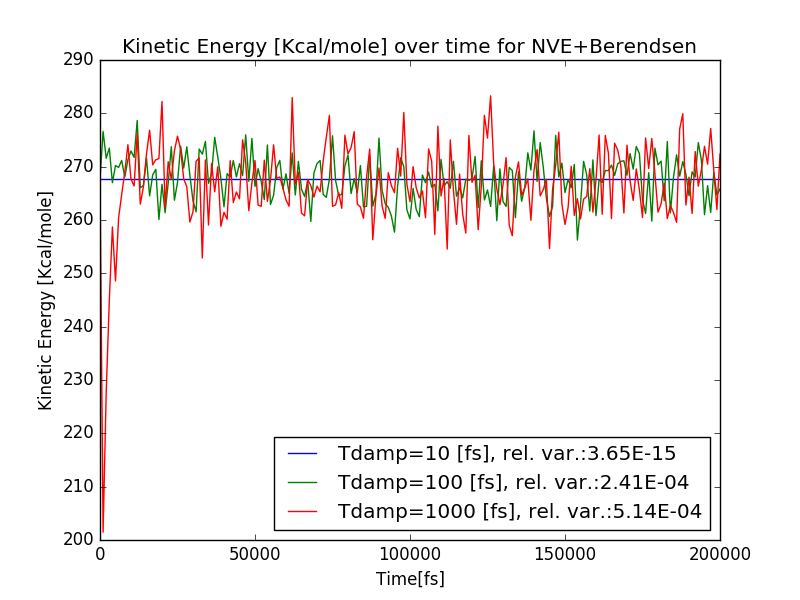
\includegraphics[width=0.5\textwidth]{\fullpathpartone/plots/dampstudy/NVEBer_KinEng_atomnum500.png}
\caption[aaa]{Equiulibriation of Temperature(top), Potential Energy(middle) and Kinetic Energy(bottom) for the Nose-Hoover thermostat(left) and the "weak-coupling" thermostat(right). The equilibriation is plotted for different damping parameters and the relative variance of the equilibriated part is provided.}
\label{fig:p1_equilibriation}
\end{figure}
\end{center}


\subsection{Stability comparison between Noose-Hoover and Berendsen}
A comparison between the Nose-Hoover thermostat and the weakly-coupled Berendsed thermostat is provided in Figure~\ref{fig:p1_NVT_vs_NVEBer}.
Overall, one can say that the weakly-coupled Berendsen delivers more accurate and stable results. Also, it does not benefit from damping, on the contrary, the relative variance increases with an increasing damping parameter.

\begin{center}
\begin{figure}[h]
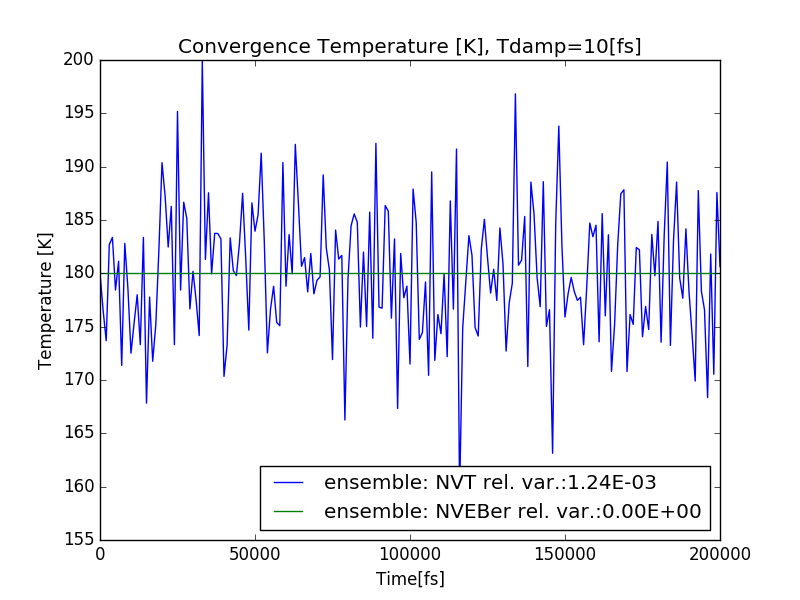
\includegraphics[width=0.5\textwidth]{\fullpathpartone/plots/NVT_vs_NVEBer/Temp_damp10_atomnum500.png}~
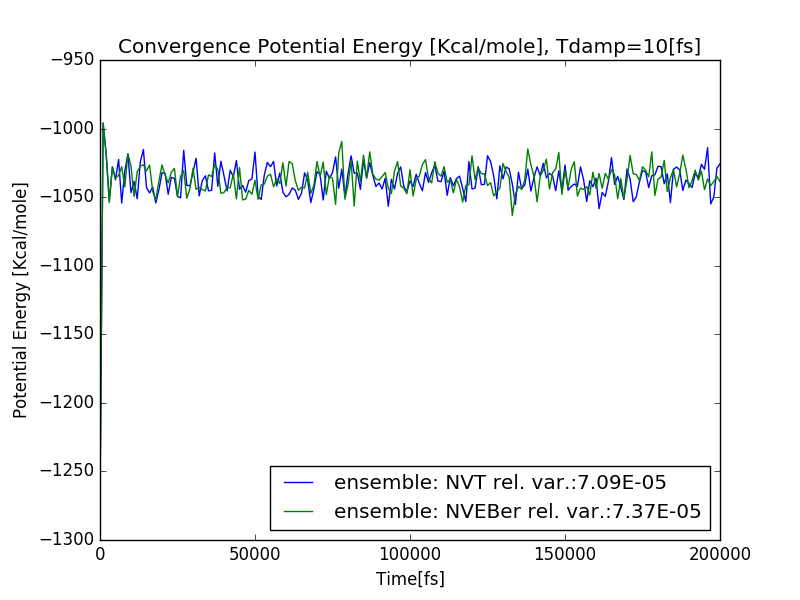
\includegraphics[width=0.5\textwidth]{\fullpathpartone/plots/NVT_vs_NVEBer/PotEng_damp10_atomnum500.png}
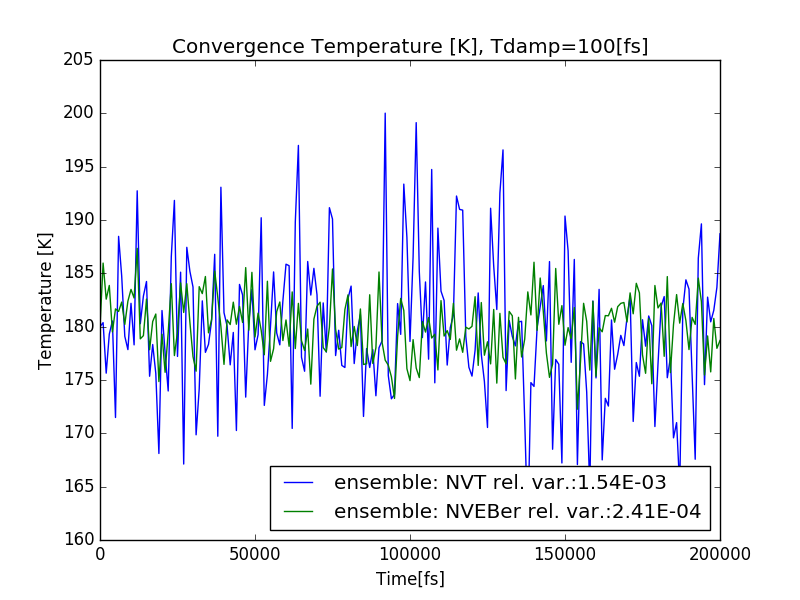
\includegraphics[width=0.5\textwidth]{\fullpathpartone/plots/NVT_vs_NVEBer/Temp_damp100_atomnum500.png}~
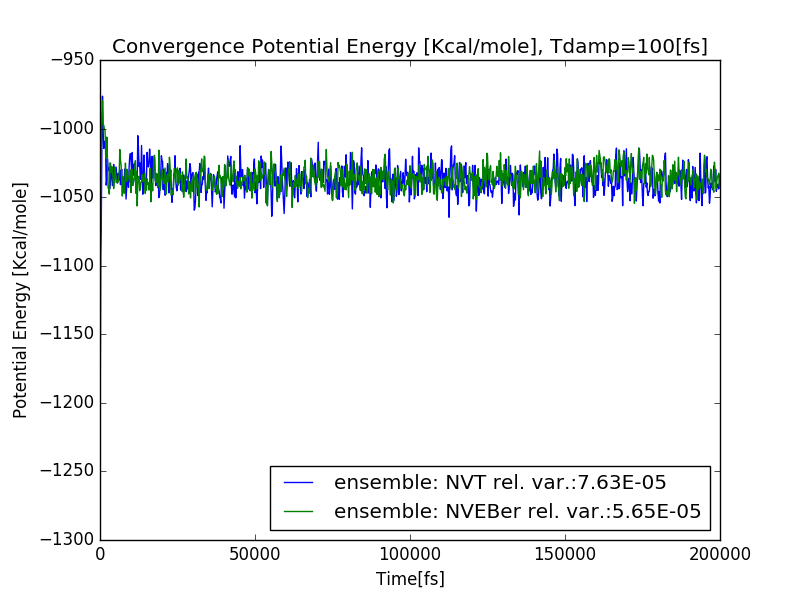
\includegraphics[width=0.5\textwidth]{\fullpathpartone/plots/NVT_vs_NVEBer/PotEng_damp100_atomnum500.png}
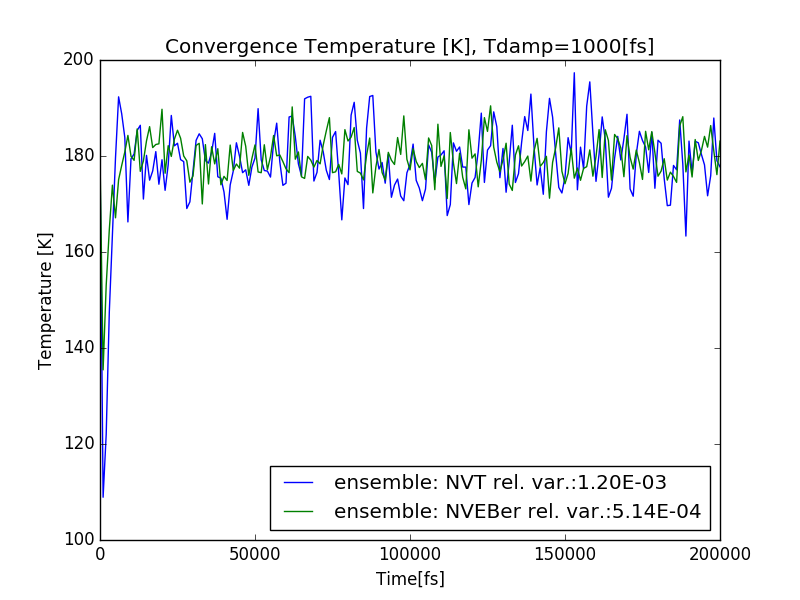
\includegraphics[width=0.5\textwidth]{\fullpathpartone/plots/NVT_vs_NVEBer/Temp_damp1000_atomnum500.png}~
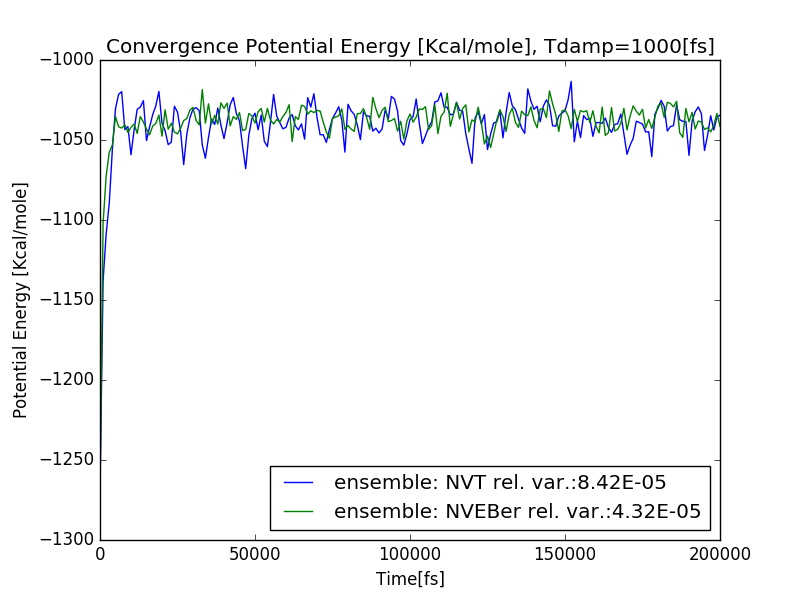
\includegraphics[width=0.5\textwidth]{\fullpathpartone/plots/NVT_vs_NVEBer/PotEng_damp1000_atomnum500.png}
\caption[aaa]{Comparions between Nose-Hoover thermostat(blue) and weakly-coupled Berendsen(green) for temperature (left) and Potential Energy(right). The 3 rows show the convergence for 3 different damping parameters.}
\label{fig:p1_NVT_vs_NVEBer}
\end{figure}
\end{center}


\subsection{Dependece on the system-size}
To determine the dependence of the Nose-Hoover thermostat's convergence on the system size, simulations with a boxsize of 5, 6, 7, 8, 9, 10, 11 and 12 have been carried out, which correlates to a total number of atoms of 500, 864, 1372, 2048, 2916, 4000, 5324 and 6912. The results are visualized in Figure~\ref{fig:p1_cellnum_study}. It can be observed, that the relative variance decays with the system size as $\frac{<T^2>-<T>^2}{<T>^2}\sim\frac{1}{N}$.

\begin{center}
\begin{figure}[h]
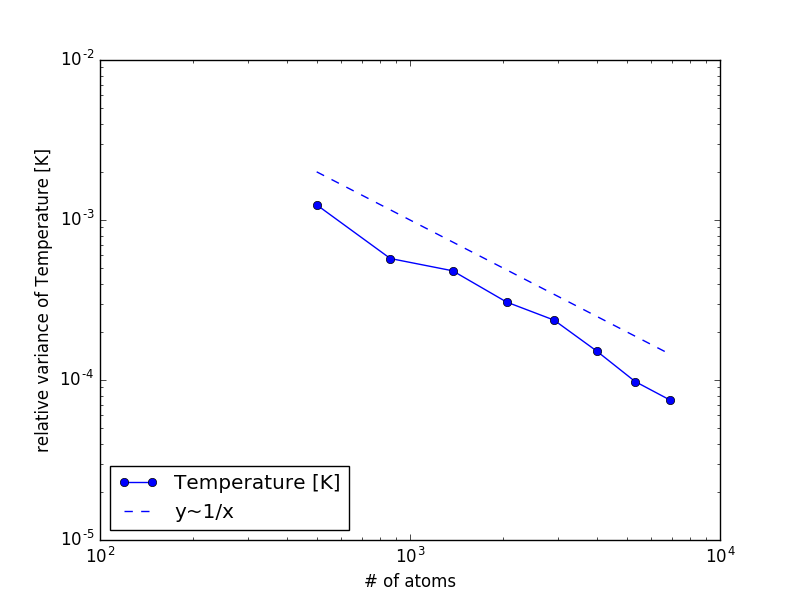
\includegraphics[width=0.5\textwidth]{\fullpathpartone/plots/cellnum_study/NVT_Temp_damp10.png}
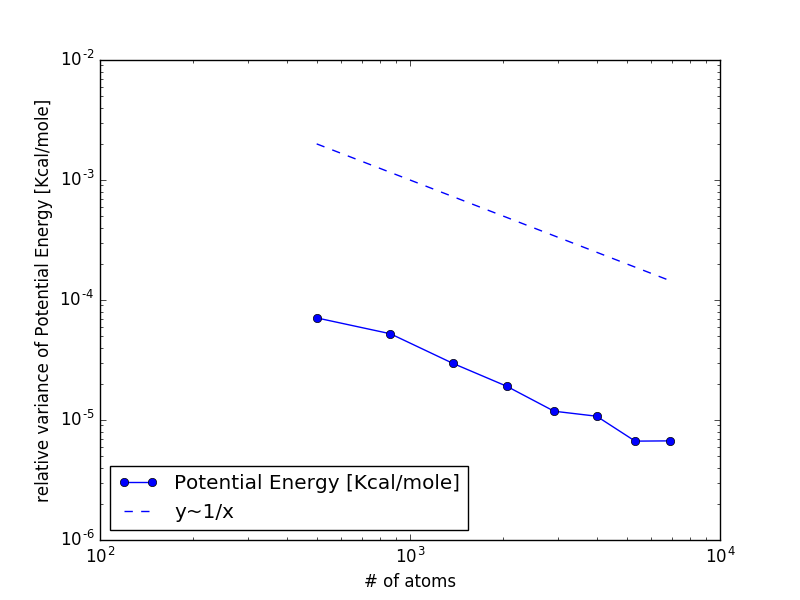
\includegraphics[width=0.5\textwidth]{\fullpathpartone/plots/cellnum_study/NVT_PotEng_damp10.png}
\caption[aaa]{Relative variance of Temperature(left) and Potential Energy(right) with respect to the number of atoms in the simulation. As the dashed line shows, the relative variance decays with the system size as $\frac{<T^2>-<T>^2}{<T>^2}\sim\frac{1}{N}$.}
\label{fig:p1_cellnum_study}
\end{figure}
\end{center}


\subsection{MCMC}







\section{Constant pressure/temperature molecular dynamics}
\subsection{Finding the equilibrium box sizes}
To determine the equilbrium box sizes, a regular simulation has been conducted and the final, equilbrium average has been used as a mean value. This is viualized in Figure~\ref{fig:p1_boxsize}. By dividing the final boxlength by the original, one can obtain a scaling factor that is applied to the following simulations via the "change\_box" command(\href{\pathpartone/in.NPT_boxmod_template}{in.NPT\_boxmod\_template}).
As a verification, the box-size is again plotted over time in the right hand side of Figure~\ref{fig:p1_boxsize}.\\

In Figure~\ref{fig:pressure_over_boxsize}, the pressure distribution of the scaled simulation is plotted for different box sizes. We can clearly see a normal-like distribution centered around the target value of 1.0 atm and a shrinking variance with increasing system size.\\
The dependency of the relative variance on the number of atoms is also plotted in the bottom two figures. Clearly, the relative variance decays invers proportional with the system size.\\
 \\
From the LAMMPS manual, we can see that the pressure is computes via the formula
\begin{align}
P=\frac{N k_B T}{N}+\frac{\sum_i^{N'}r_i\cdot f_i}{dV}
\end{align}
where $N$ is the number of atoms $k_B$ is the Boltzmann constant, $T$ is the Temperature and $V$ is the control volume. The second term contains all interactions where $r_i$ and $f_i$ are the position vector if atom $i$ and dV is the change rate of the control volume. Since we are in equilibrium, the control volume remains constant, the second term can thus be neglected. Also, in the first term, $\frac{N}{V}$ is related to the density and also constant. We can therfore expect the convergence to be of the same rate as the convergence of $T$ which has already been shown in the first part to be of first order.


\begin{center}
\begin{figure}[h]
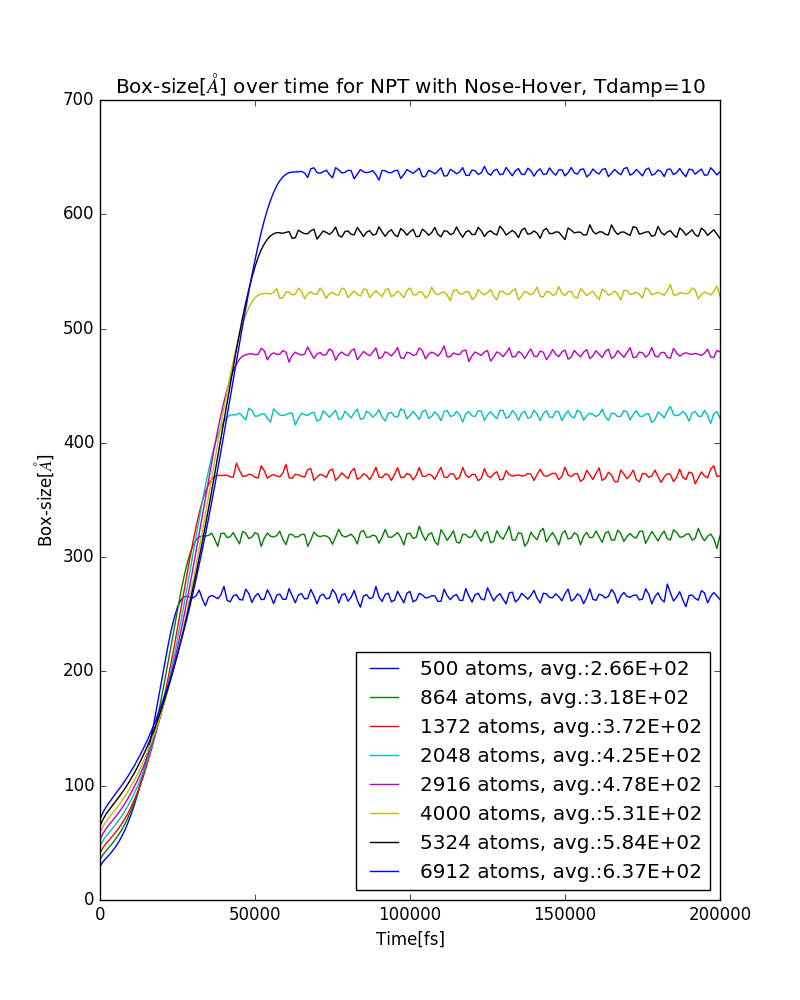
\includegraphics[width=0.5\textwidth]{\fullpathpartone/plots/boxsizesim/NPT_Lx_damp10.png}~
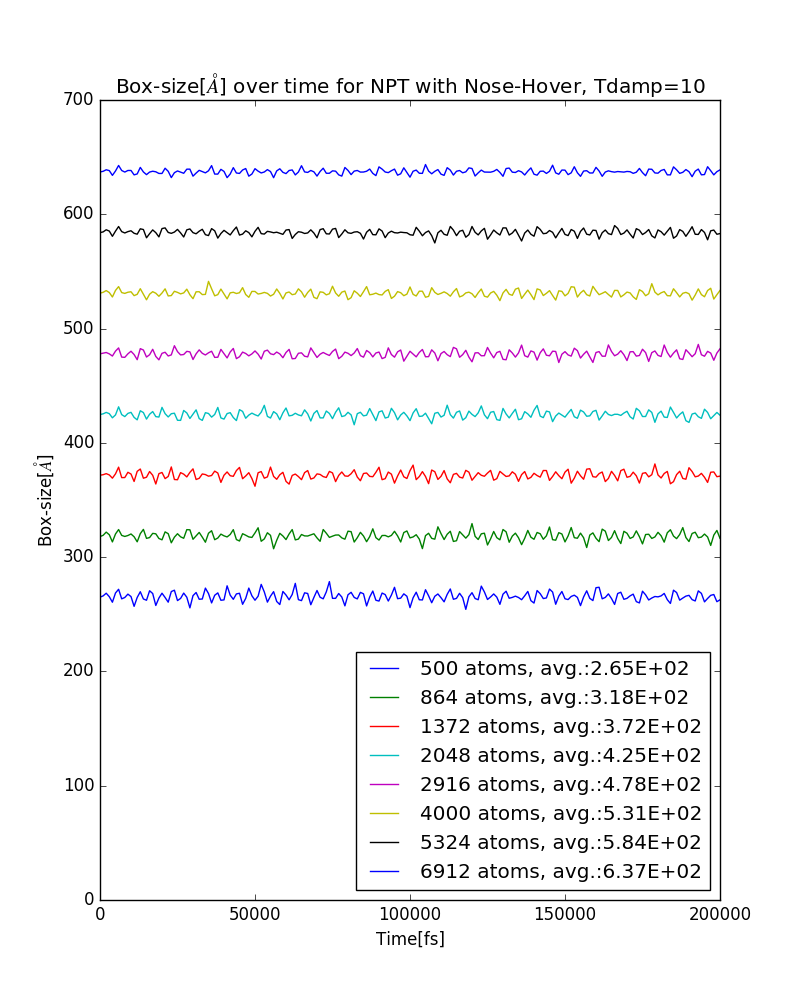
\includegraphics[width=0.5\textwidth]{\fullpathpartone/plots/boxsizesim/boxmod_NPT_Lx_damp10.png}
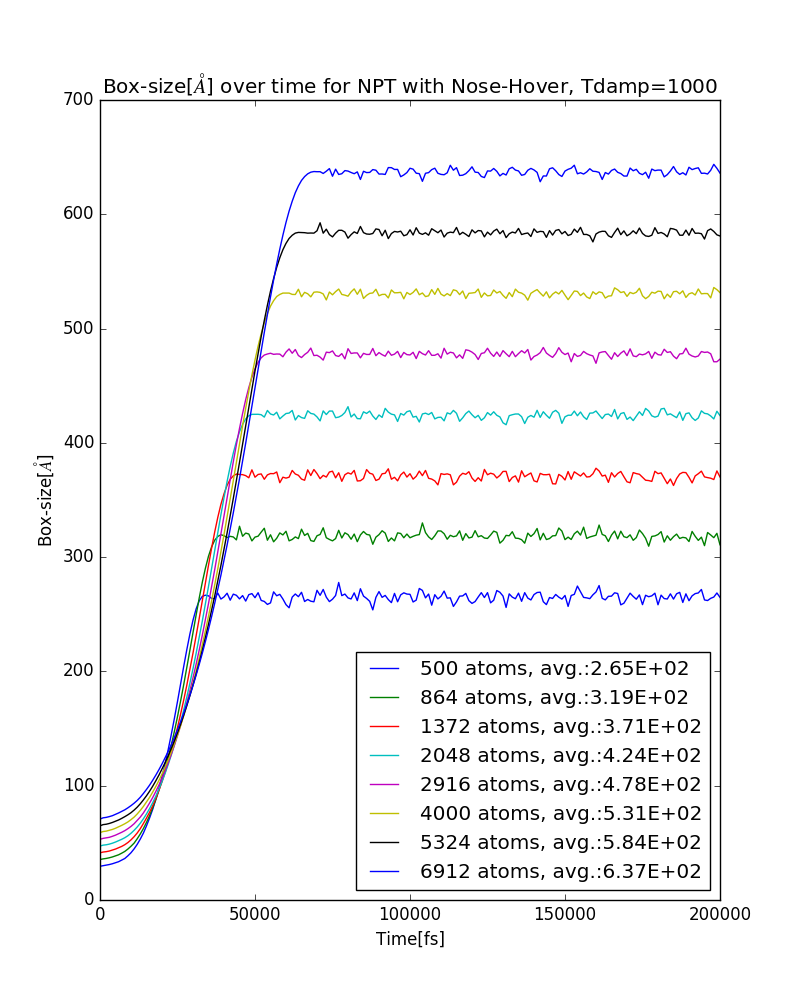
\includegraphics[width=0.5\textwidth]{\fullpathpartone/plots/boxsizesim/NPT_Lx_damp1000.png}~
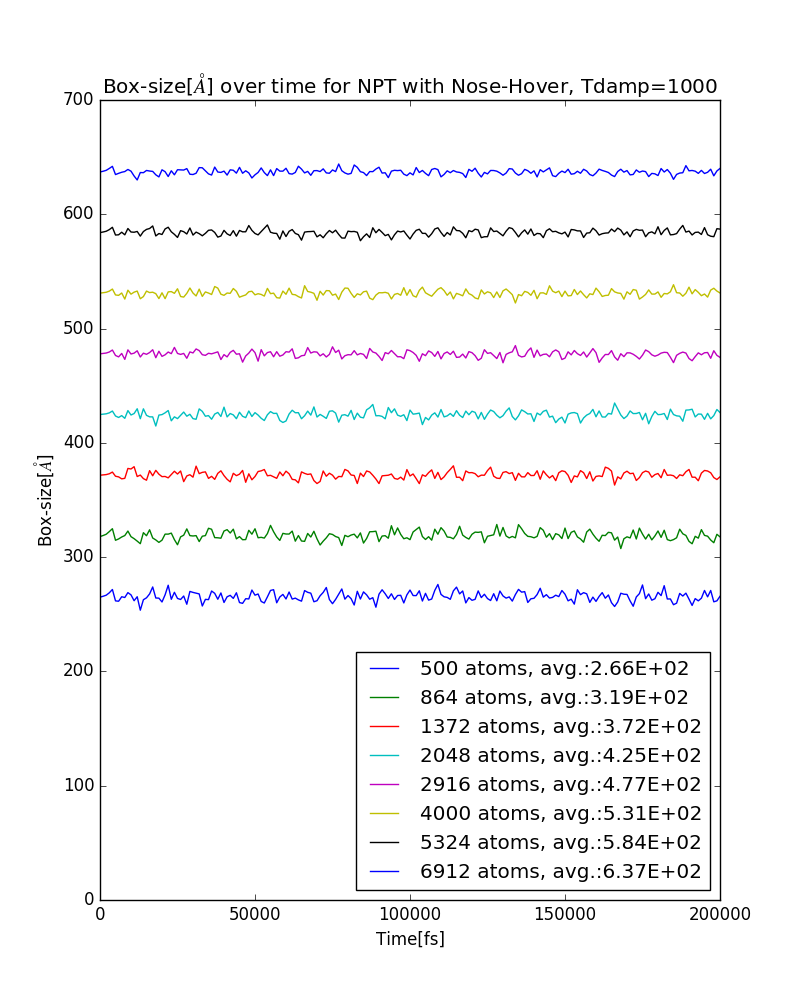
\includegraphics[width=0.5\textwidth]{\fullpathpartone/plots/boxsizesim/boxmod_NPT_Lx_damp1000.png}
\caption[aaa]{Determination of the boxsize by equilibriation(left) and Time convergence after box-size modification (right). }
\label{fig:p1_boxsize}
\end{figure}
\end{center}


\begin{center}
\begin{figure}[h]
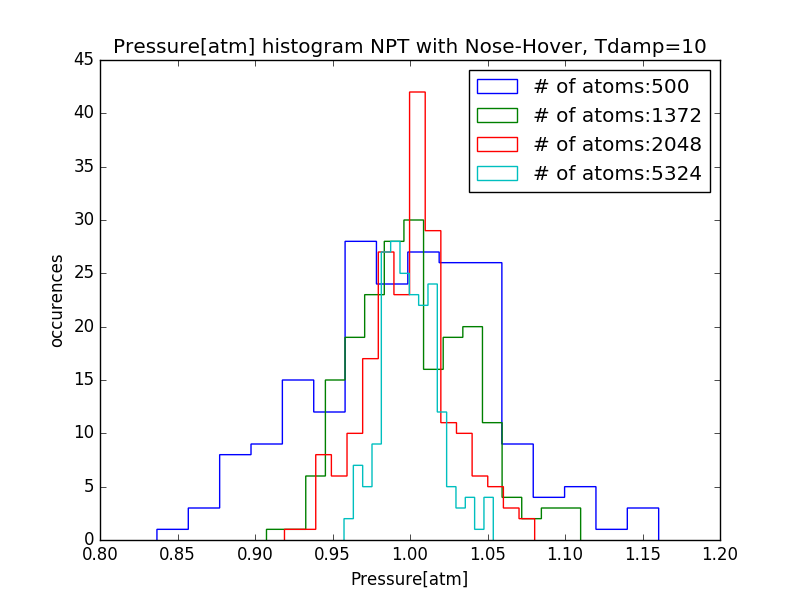
\includegraphics[width=0.5\textwidth]{\fullpathpartone/plots/boxsizesim/boxmod_NPT_Press_damp10.png}~
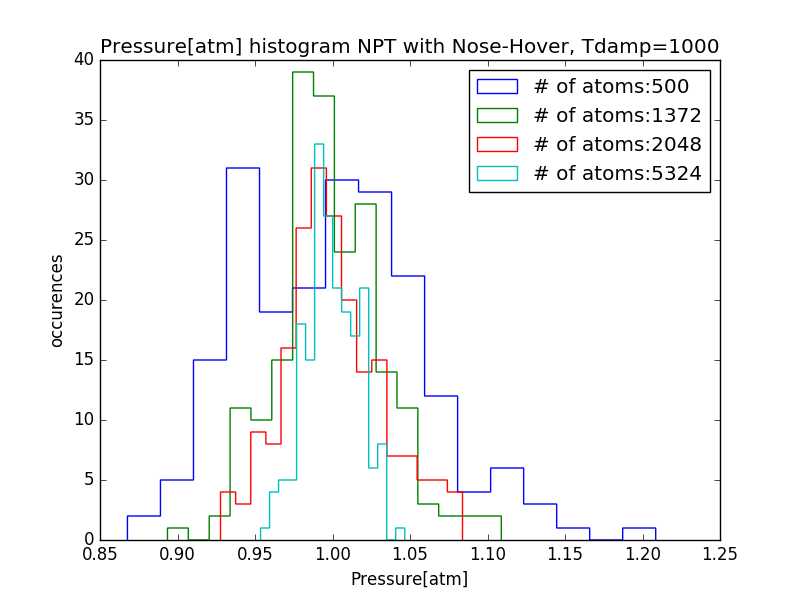
\includegraphics[width=0.5\textwidth]{\fullpathpartone/plots/boxsizesim/boxmod_NPT_Press_damp1000.png}
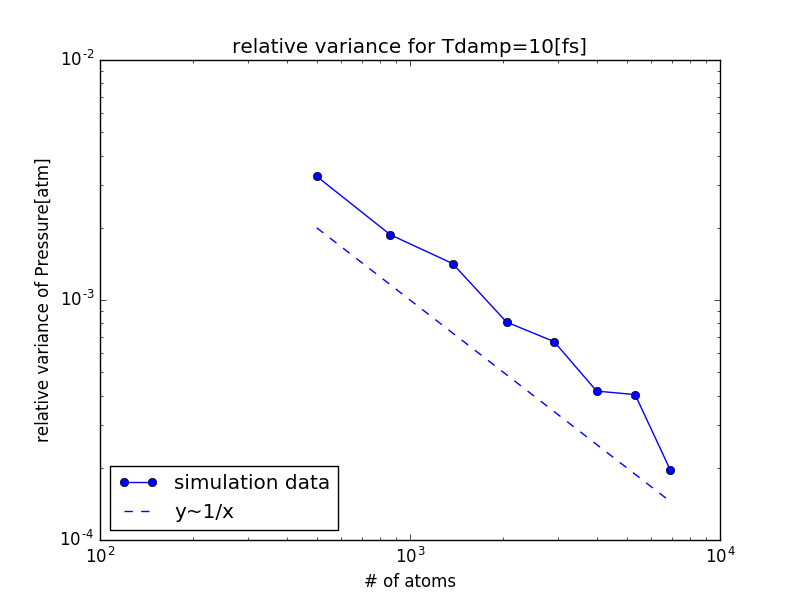
\includegraphics[width=0.5\textwidth]{\fullpathpartone/plots/boxsizesim/relvar_Press_damp10.png}~
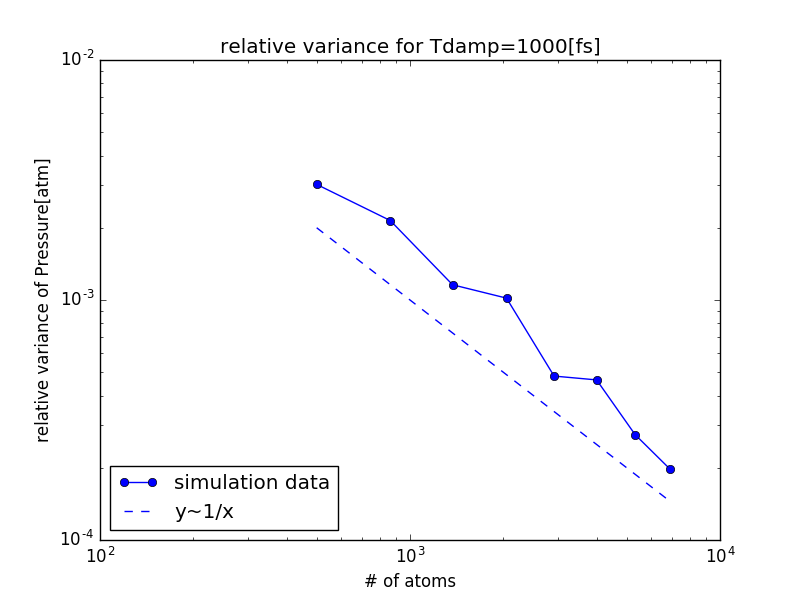
\includegraphics[width=0.5\textwidth]{\fullpathpartone/plots/boxsizesim/relvar_Press_damp1000.png}
\caption[aaa]{Influence of the system size on the simulation. The top two figures show histograms of the obtained pressure values, the bottom two figures show the dependencey of the relative variance on the system size. The left two figures have been calculated with a dampin value of $10 fs$ the right two with $1000 fs$.}
\label{fig:pressure_over_boxsize}
\end{figure}
\end{center}




\subsubsection{Prove of equilibrium}
a
\subsubsection{Stability of tghe two algorithms}
a
\subsection{Nose-Hoover dependency on system size}
a
\subsection{MCMC}
a


\section{Constant pressure/temperature thermostats}
a
\subsection{Equilibrium box size with NPT esemble}
a
\subsubsection{Noose-Hoover barostat}
a
\subsubsection{Relative pressure variance}
a
\subsubsection{Density calculation}
a
\subsection{CValculation of specific heat capacity}
a
\subsubsection{Equilibrium calculation}
a
\subsubsection{Estimation of equilibrium box length}
a
\subsubsection{Equilibroium in NVT esmeble}
a
\subsubsection{Specific heat capacity for constatn volume}
a

\section{Phase transition of Krypton}
a


\chapter{Two-dimensional tensile test}
\section{Equilibriation}
\subsection{2.1.1}
a
\subsection{2.1.2}
a

\section{Tensile test}
a















%\begin{align}
%	\rho \frac{\partial \boldsymbol{v}}{\partial t} + \nabla p =0 \label{eq:e1}          \\
%	\frac{1}{c^2} \frac{\nabla p}{t} + \rho \nabla \cdot \boldsymbol{v} =0 \label{eq:e2} 
%\end{align}
%\newline
%The normal form, provided in the lecture notes reads
%\begin{align}
%	\frac{\partial u}{\partial t}+D(f(u))=0 \label{eq:genereral_problem} 
%\end{align}
%\newline
%One can quickly see, that Equations~\ref{eq:e1}-\eqref{eq:e2} can be fitted into Eqaution \eqref{eq:genereral_problem} by defining
%
%\begin{align}
%	\boldsymbol{u}=
%	\left( \begin{array}{c}
%	\boldsymbol{v}\\
%	p
%	\end{array} \right),
%	D:=
%	\left( \begin{array}{cc}
%	\nabla\cdot             & 0              \\
%	0                       & \nabla         
%	\end{array} \right),
%	\boldsymbol{A}:=
%	\left( \begin{array}{cc}
%	0                       & \frac{1}{\rho} \\
%	\rho c^2 \boldsymbol{I} & 0              
%	\end{array} \right),
%	f\left(\boldsymbol u \right)=\boldsymbol{A}\boldsymbol{u}
%\end{align}
%\newline
%for the particular simple 1-dimensional case of this problem, one thus gets
%\begin{align}
%	\boldsymbol{u}=
%	\left( \begin{array}{c}
%	v\\
%	p
%	\end{array} \right),
%	D:=
%	\left( \begin{array}{cc}
%	\frac{\partial}{\partial x}\cdot & 0                           \\
%	0                                & \frac{\partial}{\partial x} 
%	\end{array} \right),
%	\boldsymbol{A}:=
%	\left( \begin{array}{cc}
%	0                                & \frac{1}{\rho}              \\
%	\rho c^2                         & 0                           
%	\end{array} \right)\label{eq:1D_definitions}
%\end{align}
%
%\subsection*{One-dimensional discretization}
%All furhther considerations are restricted to the 1D-case described in Equations~\eqref{eq:genereral_problem} and \eqref{eq:1D_definitions}.
%\newline
%For the Galerkin approximation, test functions are defined as follows
%
%\begin{align}
%	\boldsymbol{w}=                                                                            
%	\left( \begin{array}{c}                                                                    
%	w1                                                                                         \\
%	w2                                                                                         
%	\end{array} \right)~\left\{w \in H^1(\Omega),\ w = 0\ \text{on}\ \partial \Omega_D\right\} 
%\end{align}
%\\
%\\
%One thus gets
%\begin{align}
%	\Bd{u_t}{w}+\Bd{D(f(u))}{w}=0 
%\end{align}
%\\
%\\
%partial integration leads to
%\begin{align}
%	\Bd{u_t}{w}-\Bd{f(u)}{D(w)}+\Bb{f*(u)}{G w}=0\\
%	G=\left(\begin{matrix}
%	\hat{n} & 0             \\
%	0       & \hat{n} \cdot 
%	\end{matrix}\right)
%\end{align}
%
%where $f^*$ is the so-called "numerical flux", which simply is the value for $f(u)$ taken at the interface. Since in the DG context, this value differes from one adjacent element to the other, a rule must be found to decide upo a certain value. The flux will choice and derivation of an approriate flux will be treated later.
%
%In the 1D case, the above equation can be written as
%\begin{align}
%	\Bd{u}{w}-\Bd{f(u)}{D w}+f^*(u)^T\mathop{\Bigg|}\limits_{x_k}^{x_{k+1}} \boldsymbol I=0\label{eq:weak_form_1D} 
%\end{align}
%
%The problem is now discretized with a Bubnov-Galerkin scheme,so
%\begin{align}
%	w_h=\sum_{k=1}^N \dmat{\phi_k} \dvec {w_k} \\
%	u_h=\sum_{k=1}^N \dmat{\phi_k} \dvec {u_k} 
%\end{align}
%are the approximation to the shape-function and the test-function.
%
%In the above equations, one still has to take into account, that $u$ consists of the two independent variables $v$ and $p$. Therefor, they have to be weighted and tested independently.We can thus write:
%
%
%\begin{align}
%	w_h=\sum_{k=1}^N 
%	\begin{bmatrix}
%	\phi_k^1 & 0        \\
%	0        & \phi_k^2 
%	\end{bmatrix}\cdot
%	\begin{bmatrix}
%	w_k^1\\
%	w_k^2
%	\end{bmatrix}=\sum_{k=1}^N 
%	\dmat{\phi_k} \cdot \dvec{w_k}
%	\\
%	u_h=\sum_{k=1}^N 
%	\begin{bmatrix}
%	\phi_k^1 & 0        \\
%	0        & \phi_k^2 
%	\end{bmatrix}\cdot
%	\begin{bmatrix}
%	u_k^1\\
%	u_k^2
%	\end{bmatrix}=\sum_{k=1}^N 
%	\dmat{\phi_k} \cdot \dvec{u_k}
%\end{align}
%
%The shape-functions $\dmat{\phi_k}$ are taken as Lagrange-polynomials based on Gauss-Lobatto points. For the purpose of this report, shape-functions up to a degree of 10 have been implemented.
%
%By inserting the above ansatz into the weak form provided in~\eqref{eq:weak_form_1D}, on can thus derive the following matrix notation:
%\begin{align}
%	\dmat{M} \dvec{\ddot{\dvec{u}}} + (-\dmat{S}+\dmat{F}) \dvec{u} & = \dmat{-F_{bound}} \dvec{h}\text{ where e.g.} \\
%	\dmat{M_{ij}}                                                   & =(\dmat{\phi_i},\dmat{\phi_j})                 
%\end{align}
%Since $\dmat{\phi_i}$ has a 2x2 matrix shape, the full $\dmat{M}$ matrix consists of diagonal 2x2 blocks assembled through the dof numbering sheme as depicted in Figure~\ref{fig:dof_numbering}.
%The element matrix genaration can be formaulated in matrixform as:
%\begin{align}
%	\dmat{M_k} & =\int_{D^k} \dmat{N} \dmat{N}^T det(\dmat{J}) d\xi                                                \\
%	\dmat{S_k} & =\int_{D^k} \dmat{D} \dmat{N} \dmat{A} \dmat{N}^T \dmat{J}^{-1} det{\dmat{J}} d\xi\text{,  where} \\
%	\dmat{N}   & =                                                                                                 
%	\begin{bmatrix}
%	\phi_k^1   & 0                                                                                                 \\
%	0          & \phi_k^2                                                                                          \\
%	\vdots     & \vdots                                                                                            \\
%	\phi_k^n   & 0                                                                                                 \\
%	0          & \phi_k^n                                                                                          
%	\end{bmatrix}
%\end{align}
%
%\subsection*{F-matrix}
%The derivation of the flux-matrix $\dmat{F}$ is somewhat more difficult. We consider the last term of the wek form given in~\eqref{eq:weak_form_1D}. Clearly the resulting matrix depends on the definition of $f^*$. For this report, the Lax-Friedrichs(LF) and the  Hydrizable Discontinous Galerkin(HDG) flux were considered.
%\subsubsection{Lax-Friedrich flux}
%The Lax Friedrich flux is defined as
%\begin{align}
%	f^{*,LF}(u^+,u^-)=\frac{f(u^-)+f(u^+)}{2}+\frac{C}{2} \boldsymbol{\hat{n}}^{-} (u^- -u^+) 
%\end{align}
%where $u^-$ denotes the u value of the current element and $u^+$ denotes the $u$ value of the neigbour.
%
%The Flux matrix shall be exemplarily derived by looking at one elmenet $k$ as described in Figure~\ref{fig:ele_setup}.
%\paragraph{Left Node}
%\begin{align}
%	u^+=\left(\begin{array}{c} v_{k-1}^2 \\p_{k-1}^2 \end{array}\right),
%	u^-=\left(\begin{array}{c} v_{k}^1   \\p_{k}^1 \end{array}\right),
%	\hat{n}^{-}=-1                       
%\end{align}
%
%\begin{align}
%	f^{*,LF}(x_k) & = 
%	\frac{
%	\dmat{A_{k}}   \left(\begin{array}{c} v_{k}^1\\p_{k}^1 \end{array}\right)+
%	\dmat{A_{k-1}} \left(\begin{array}{c} v_{k-1}^2\\p_{k-1}^2 \end{array}\right)  
%	}{2} -
%	\frac{ 
%	C_{k}   \left(\begin{array}{c} v_{k}^1\\p_{k}^1 \end{array}\right) -
%	C_{k-1} \left(\begin{array}{c} v_{k-1}^2\\p_{k-1}^2 \end{array}\right) 
%	}{2} \\
%	              & = 
%	\frac{1}{2}(\dmat{A_k}-C_k\dmat{I}) \left(\begin{array}{c} v_{k}^1\\p_{k}^1 \end{array}\right) +
%	\frac{1}{2}(\dmat{A_{k-1}}+C_{k-1}\dmat{I}) \left(\begin{array}{c} v_{k-1}^2\\p_{k-1}^2 \end{array}\right)
%\end{align}
%
%
%
%
%\paragraph{Right Node}
%\begin{align}
%	u^+=\left(\begin{array}{c} v_{k+1}^1 \\p_{k+1}^1 \end{array}\right),
%	u^-=\left(\begin{array}{c} v_{k}^2   \\p_{k}^2 \end{array}\right),
%	\hat{n}^{-}=1                        
%\end{align}
%
%\begin{align}
%	f^{*,LF}(x_k) & = 
%	\frac{
%	\dmat{A_{k}}   \left(\begin{array}{c} v_{k}^2\\p_{k}^2 \end{array}\right)+
%	\dmat{A_{k-1}} \left(\begin{array}{c} v_{k+1}^1\\p_{k+1}^1 \end{array}\right)  
%	}{2} +
%	\frac{ 
%	C_{k}  \left(\begin{array}{c} v_{k}^2\\p_{k}^2 \end{array}\right) -
%	C_{k-1} \left(\begin{array}{c} v_{k+1}^1\\p_{k+1}^1 \end{array}\right) 
%	}{2} \\
%	              & = 
%	\frac{1}{2}(\dmat{A_k}+C_k\dmat{I})         \left(\begin{array}{c} v_{k}^2\\p_{k}^2 \end{array}\right) +
%	\frac{1}{2}(\dmat{A_{k+1}}-C_{k+1}\dmat{I}) \left(\begin{array}{c} v_{k+1}^1\\p_{k+1}^1 \end{array}\right)
%\end{align}
%
%
%So as a whole, for the boundary integral in Equation~\eqref{eq:weak_form_1D} the following term can be derived
%\begin{align}
%	\begin{split}
%	f^{*,LF}(x_{k+1})-f^{*,LF}(x_{k})=
%	  &   
%	\frac{1}{2}(\dmat{A_k}+C_k\dmat{I})         \left(\begin{array}{c} v_{k}^2\\p_{k}^2 \end{array}\right) +
%	\frac{1}{2}(\dmat{A_{k+1}}-C_{k+1}\dmat{I}) \left(\begin{array}{c} v_{k+1}^1\\p_{k+1}^1 \end{array}\right)
%	\\
%	- &   
%	\frac{1}{2}(\dmat{A_k}-C_k\dmat{I}) \left(\begin{array}{c} v_{k}^1\\p_{k}^1 \end{array}\right) -
%	\frac{1}{2}(\dmat{A_{k-1}}+C_{k-1}\dmat{I}) \left(\begin{array}{c} v_{k-1}^2\\p_{k-1}^2 \end{array}\right)
%	\end{split}
%\end{align}
%
%\vspace{3cm}
%
%\begin{figure}[h!]
%	\begin{center}
%		\begin{tikzpicture}
%			    
%			\draw [thick,dashed] (0,0) -- (1,0);
%			\draw [thick](1,0) -- (5,0);
%			\draw [thick,dashed] (5,0) -- (6,0);
%			      
%			\draw [thick,black,fill=white] (1,0) circle [radius=0.1] node [black,below=4]{$\left(\begin{array}{c} v_k^1=u_k^1\\p_k^1=u_k^2 \end{array}\right) $}; % Draws a circle
%			\draw [thick,black,fill=white] (3,0) circle [radius=0.1] node [black,below=4]{$\left(\begin{array}{c} v_k^2=u_k^3\\p_k^2=u_k^4 \end{array}\right) $}; % Draws a circle
%			\draw [thick,black,fill=white] (5,0) circle [radius=0.1] node [black,below=4]{$\left(\begin{array}{c} v_k^3=u_k^5\\p_k^3=u_k^6 \end{array}\right) $}; % Draws a circle
%			        
%			
%			    
%		\end{tikzpicture}
%		\caption[short caption]{Dof numbering convention for the 1D-example}
%		\label{fig:dof_numbering}
%	\end{center}
%\end{figure}
%
%
%\begin{figure}[h!]
%	\begin{center}
%		\begin{tikzpicture}
%			    
%			\draw [thick,dashed] (0,1) -- (1,1);
%			\draw [thick](1,1) -- (3,1);
%			\draw [thick](3,0) -- (7,0);
%			\draw [thick](7,1) -- (9,1);
%			\draw [thick,dashed] (9,1) -- (10,1);
%			        
%			\draw [thick,black,fill=white] (3,1) circle [radius=0.1] node [black,above=4]{$\left(\begin{array}{c} v_{k-1}^2\\p_{k-1}^2 \end{array}\right) $}; % Draws a circle
%			\draw [thick,black,fill=white] (3,0) circle [radius=0.1] node [black,below=4]{$\left(\begin{array}{c} v_{k}^1\\p_{k}^1 \end{array}\right) $}; % Draws a circle
%			\draw [thick,black,fill=white] (7,1) circle [radius=0.1] node [black,above=4]{$\left(\begin{array}{c} v_k^1\\p_k^1 \end{array}\right) $}; % Draws a circle
%			\draw [thick,black,fill=white] (7,0) circle [radius=0.1] node [black,below=4]{$\left(\begin{array}{c} v_k^2\\p_k^2 \end{array}\right) $}; % Draws a circle
%			      
%			%\draw (7,2) node {$\left(\begin{array}{c} v_k^1\\p_k^1 \end{array}\right) $};
%			%\draw (3,2) node {$\left(\begin{array}{c} v_{k-1}^2\\p_{k-1}^2 \end{array}\right) $};
%			      
%			%\draw (7,-1) node {$\left(\begin{array}{c} v_k^2\\p_k^2 \end{array}\right) $};
%			%\draw (3,-1) node {$\left(\begin{array}{c} v_{k}^1\\p_{k}^1 \end{array}\right) $};
%			      
%			\draw (5,0) node {\colorbox{white}{$k$}};
%			\draw (2,1) node {\colorbox{white}{$k-1$}};
%			\draw (8,1) node {\colorbox{white}{$k+1$}};
%			    
%		\end{tikzpicture}
%		\caption[short caption]{Element notation}
%		\label{fig:ele_setup}
%	\end{center}
%\end{figure}
%
%
%\chapter*{Tasks}
%\section*{Task1}
%The derivation of the local Lax-Friedrich flux has been carried out above.
%\section*{Task2}
%A formula for calculation of the timestep is provided in the lecture notes. Substitution, according to our Notation leads to:
%\begin{align}
%	\Delta t \leq K \frac{h}{p^2 c}\label{eq:timestep}        
%\end{align}     
%Here, K denotes a constant that is independent from the discretization. It depends only on the equation at hand, as well as the time integration method, and can thus be found easily by numerical experiments.
%\section*{Task3}
%
%The setup for task 3 is shown in Figure \ref{fig:setup3}. The simulation has been carried out with an timestep obtained by Equation~\eqref{eq:timestep}. As Figures~\ref{fig:error_development}-\ref{fig:task3_flux_comparison} show, the convergence order can be improved by using higher order polynomials, as expected. In general, the Lax-Friedrich flux deliverd slightly better results than the HDG-flux.
%
%\begin{figure}[h]
%	\begin{center}
%		\begin{tikzpicture}
%			\draw [thick] (0,0) -- (9,0);
%			 
%			\draw [thick,black,fill=white] (0,0) circle [radius=0.1] node [black,below=4]{$x=0$};
%			\draw [thick,black,fill=white] (9,0) circle [radius=0.1] node [black,below=4]{$x=1$};
%			    
%			\node[anchor=base, align=left] at (4.5,0.2){$\rho=1$\\$c=1$};
%		\end{tikzpicture}
%	\end{center}
%	\caption[short caption]{Setup for task 3. Both parameters $\rho$ and $c$ are constant in the whole domain. }
%	\label{fig:setup3}
%\end{figure}
%
%
%\begin{figure}[h]
%	\begin{center}
%		\begin{tikzpicture}
%			
%			\begin{semilogyaxis}[xlabel={$time$},ylabel={$\epsilon_p$}, grid=major,width=12cm,height=7cm, legend pos=outer north east,cycle list name=elelist]
%				
%				\addplot+[style=solid,very thick] table [skip first n=1,x index=0, y index=1, col sep=comma]
%				{\resultspath/config_task3_K5_N1_LF_tend6/L2err_P.dat};
%				\addlegendentry{5 elements}
%				
%				\addplot+[style=solid,very thick] table [skip first n=1,x index=0, y index=1, col sep=comma]
%				{\resultspath/config_task3_K10_N1_LF_tend6/L2err_P.dat};
%				\addlegendentry{10 elements}
%					  
%				\addplot+[style=solid,very thick] table [skip first n=1,x index=0, y index=1, col sep=comma]
%				{\resultspath/config_task3_K20_N1_LF_tend6/L2err_P.dat};
%				\addlegendentry{20 elements}
%					  
%				\addplot+[style=solid,very thick] table [skip first n=1,x index=0, y index=1, col sep=comma]
%				{\resultspath/config_task3_K40_N1_LF_tend6/L2err_P.dat};
%				\addlegendentry{40 elements}
%					  
%				\addplot+[style=solid,very thick] table [skip first n=1,x index=0, y index=1, col sep=comma]
%				{\resultspath/config_task3_K80_N1_LF_tend6/L2err_P.dat};
%				\addlegendentry{80 elements}	  
%				
%			\end{semilogyaxis}
%			
%		\end{tikzpicture}
%	\end{center}
%	\caption[short caption]{Development of the integral L2-error of $p$ for the setup described in \ref{fig:setup3} from $t=0$ to $t=6$}
%	\label{fig:error_development}
%\end{figure}
%
%\begin{figure}[h]
%	\begin{center}
%		\begin{tikzpicture}
%			\begin{groupplot}[
%					group style={group size=2 by 1,
%						horizontal sep = 2.95cm,
%						vertical sep = 3 cm,
%					},
%					height=7cm,width=7cm,
%					ylabel=$\varepsilon$,
%					ylabel near ticks,
%					ymode=log,
%					legend pos=outer north east,
%				cycle list name = exotic]
%				\nextgroupplot[
%					xmode=log,
%					ymode=log,
%					xlabel=numele,
%					cycle list name=convergelist
%				]
%				
%				\addplot+ table[x index=0,y index=1] {\resultspath/config_task3_convergence_N1_LF.dat};
%				\addplot+ table[x index=0,y index=1] {\resultspath/config_task3_convergence_N2_LF.dat};
%				\addplot+ table[x index=0,y index=1] {\resultspath/config_task3_convergence_N3_LF.dat};
%				\addplot+ table[x index=0,y index=1] {\resultspath/config_task3_convergence_N4_LF.dat};
%				\legend{N=1, N=2, N=3, N=4}
%				\node at (axis cs:5,1e-11) [anchor=south west] {LF};
%				      
%				\addplot[mark=none,dashed] coordinates {(10,0.5*1e-3) (100,1.58*1e-5)};
%				\node at (axis cs:50,0.3*1e-3) {$~h^{1.5}$};
%				\addplot[mark=none,dashed] coordinates {(10,0.5*1e-3) (100,1.58*1e-6)};
%				\node at (axis cs:50,0.1*1e-5) {$~h^{2.5}$};
%				\addplot[mark=none,dashed] coordinates {(10,1e-6) (100,3.1622e-10)};
%				\node at (axis cs:50,1e-8) {$~h^{3.5}$};
%				\addplot[mark=none,dashed] coordinates {(10,1e-7) (100,3.1622e-12)};
%				\node at (axis cs:50,1e-11) {$~h^{4.5}$};      
%				      
%				
%				\nextgroupplot[
%					xmode=log,
%					ymode=log,
%					xlabel=numele,
%					cycle list name=convergelist
%				]
%				\addplot+ table[x index=0,y index=1] {\resultspath/config_task3_convergence_N1_HDG.dat};
%				\addplot+ table[x index=0,y index=1] {\resultspath/config_task3_convergence_N2_HDG.dat};
%				\addplot+ table[x index=0,y index=1] {\resultspath/config_task3_convergence_N3_HDG.dat};
%				\addplot+ table[x index=0,y index=1] {\resultspath/config_task3_convergence_N4_HDG.dat};
%				\legend{N=1, N=2, N=3, N=4}
%				\node at (axis cs:5,1e-11) [anchor=south west] {HDG};
%				      
%				\addplot[mark=none,dashed] coordinates {(10,0.3*1e-2) (100,0.3*3.1622e-4)};
%				\node at (axis cs:50,1e-3) {$~h^{1.5}$};
%				\addplot[mark=none,dashed] coordinates {(10,0.1*1e-3) (100,0.1*3.1622e-6)};
%				\node at (axis cs:50,1e-5) {$~h^{2.5}$};
%				\addplot[mark=none,dashed] coordinates {(10,0.2*1e-5) (100,0.2*3.1622e-9)};
%				\node at (axis cs:50,0.51e-7) {$~h^{3.5}$};
%				\addplot[mark=none,dashed] coordinates {(10,0.3*1e-7) (100,0.3*3.1622e-12)};
%				\node at (axis cs:50,1e-10) {$~h^{4.5}$};  
%				
%			\end{groupplot}
%		\end{tikzpicture}
%	\end{center}
%	\caption[short caption]{Setup as described in Figure~\ref{fig:setup3}. The L2-error is evaluated at after 10 timesteps. The timestep was 1.0e-6. In general, we can observe, that both the HDG and the LF-flux deliver statisfying results. The expected convergence order has been obtained for all polynomial degrees.}
%	\label{fig:task3}
%\end{figure}
%
%
%
%
%\begin{figure}[h]
%	\begin{center}
%		\begin{tikzpicture}
%			
%			\begin{loglogaxis}[xlabel={$numele$},ylabel={$\epsilon_p$}, grid=major,width=12cm,height=7cm, legend pos=outer north east,cycle list name=convergelist]
%				
%				\addplot+ table[x index=0,y index=1] {\resultspath/config_task3_convergence_N1_LF.dat};
%				\addplot+ table[x index=0,y index=1] {\resultspath/config_task3_convergence_N2_LF.dat};
%				\addplot+ table[x index=0,y index=1] {\resultspath/config_task3_convergence_N3_LF.dat};
%				\addplot+ table[x index=0,y index=1] {\resultspath/config_task3_convergence_N4_LF.dat};
%				\pgfplotsset{cycle list shift=-4}
%				\addplot+[dashed] table[x index=0,y index=1] {\resultspath/config_task3_convergence_N1_HDG.dat};
%				\addplot+[dashed] table[x index=0,y index=1] {\resultspath/config_task3_convergence_N2_HDG.dat};
%				\addplot+[dashed] table[x index=0,y index=1] {\resultspath/config_task3_convergence_N3_HDG.dat};
%				\addplot+[dashed] table[x index=0,y index=1] {\resultspath/config_task3_convergence_N4_HDG.dat};
%				\legend{N=1 (LF),N=2 (LF),N=3 (LF),N=4 (LF),N=1 (HDG),N=2 (HDG),N=3 (HDG),N=4 (HDG)}
%			\end{loglogaxis}
%			
%		\end{tikzpicture}
%	\end{center}
%	\caption[short caption]{Comparison of LF and HDG flux for task 3. From this setup one can not really determine a superior flux.}
%	\label{fig:task3_flux_comparison}
%\end{figure}
%
%
%
%\begin{figure}[h]
%	\begin{center}
%		\includegraphics[width=0.9\textwidth]{\resultspath/config_task3_K200_N1_hdg.pdf}
%		\caption[short caption]{Setup as described in \ref{fig:setup3} with dirichlet boundary conditions. The x-axis shows the position, the y-axis the time. At perfectly periodic oscillation can be observed. For this plot 200 elements with a polymomial degree of 1 were used.}
%		\label{fig:task3_imagesc_hdg}
%	\end{center}
%\end{figure}
%
%
%\section*{Task4}
%
%The basic setup for task 4 is shown in Figure~\ref{fig:setup4}. The simulation has been carried oput with an timestep of $1e-6$. Figures~\ref{fig:task4_dirichlet_hdg}-\ref{fig:task4_absorbing_hdg} show the results for LF and HDG, both with Dirichlet and absorbing boundary conditions.
%
%\begin{figure}
%	\begin{center}
%		\begin{tikzpicture}
%			\draw [thick] (0,0) -- (9,0);
%			 
%			\draw [thick,black,fill=white] (0,0) circle [radius=0.1] node [black,below=4]{$x=0$};
%			\draw [thick,black,fill=white] (9,0) circle [radius=0.1] node [black,below=4]{$x=1$};
%			    
%			\node[anchor=base, align=left] at (4.5,0.2){$\rho=1.2$\\$c=340$};
%		\end{tikzpicture}
%	\end{center}
%	\caption[aaa]{Setup for task 4. Both parameters $\rho$ and $c$ are constant in the whole domain. }
%    \label{fig:setup4}
%\end{figure}
%
%
%
%
%%%%%%%%%%%%%%%%%%%%%%%%%%%%%%%%%%%%%%%%%
%\begin{figure}[h]
%	\begin{center}
%		\begin{tikzpicture}
%			
%			\begin{groupplot}[
%					group style={group size=2 by 1,
%						horizontal sep = 4.0cm,
%					},
%				height=7cm,width=7cm]
%				\nextgroupplot[
%					xlabel={t},
%					ylabel={v},
%					legend entries={t=0.0e-4,
%						t=6.0e-4,
%						t=1.2e-3,
%						t=1.8e-3,
%						t=2.4e-3,
%						t=3.0e-3},
%				legend pos=outer north east]
%				
%							
%							
%				\addlegendimage{no markers,black, dashed}			
%				\addlegendimage{no markers,s2_1}
%				\addlegendimage{no markers,s2_2}
%				\addlegendimage{no markers,s2_3}
%				\addlegendimage{no markers,s2_4}
%				\addlegendimage{no markers,s2_5}
%				
%				
%				
%				\foreach \F in {1,2,...,40}{
%					\addplot[style=solid,thick, black, dashed] table [skip first n=1,x index=0, y index=1, col sep=comma]
%					{\resultspath/config_task4_K40_N4_dirichlet_hdg/V_ele\F.dat};
%				}
%				
%				
%				\foreach \F in {1,2,...,40}{
%					\addplot[style=solid,thick, s2_1] table [skip first n=1,x index=0, y index=2, col sep=comma]
%					{\resultspath/config_task4_K40_N4_dirichlet_hdg/V_ele\F.dat};
%				}
%					
%					    
%					    
%				\foreach \F in {1,2,...,40}{
%					\addplot[style=solid,thick, s2_2] table [skip first n=1,x index=0, y index=3, col sep=comma]
%					{\resultspath/config_task4_K40_N4_dirichlet_hdg/V_ele\F.dat};
%				}
%				    
%					    
%				\foreach \F in {1,2,...,40}{
%					\addplot[style=solid,thick, s2_3] table [skip first n=1,x index=0, y index=4, col sep=comma]
%					{\resultspath/config_task4_K40_N4_dirichlet_hdg/V_ele\F.dat};
%				}
%					
%					    
%				\foreach \F in {1,2,...,40}{
%					\addplot[style=solid,thick, s2_4] table [skip first n=1,x index=0, y index=5, col sep=comma]
%					{\resultspath/config_task4_K40_N4_dirichlet_hdg/V_ele\F.dat};
%				}
%					
%					    
%				\foreach \F in {1,2,...,40}{
%					\addplot[style=solid,thick, s2_5] table [skip first n=1,x index=0, y index=6, col sep=comma]
%					{\resultspath/config_task4_K40_N4_dirichlet_hdg/V_ele\F.dat};
%				}
%					
%					
%					
%					
%				\nextgroupplot[
%					xlabel={t},
%					ylabel={p},
%				cycle list name=elelist]
%				
%				
%				\foreach \F in {1,2,...,40}{
%					\addplot[style=solid,thick, black, dashed] table [skip first n=1,x index=0, y index=1, col sep=comma]
%					{\resultspath/config_task4_K40_N4_dirichlet_hdg/P_ele\F.dat};
%				}
%				
%				
%				\foreach \F in {1,2,...,40}{
%					\addplot[style=solid,thick, s2_1] table [skip first n=1,x index=0, y index=2, col sep=comma]
%					{\resultspath/config_task4_K40_N4_dirichlet_hdg/P_ele\F.dat};
%				}
%					
%					    
%					    
%				\foreach \F in {1,2,...,40}{
%					\addplot[style=solid,thick, s2_2] table [skip first n=1,x index=0, y index=3, col sep=comma]
%					{\resultspath/config_task4_K40_N4_dirichlet_hdg/P_ele\F.dat};
%				}
%				    
%					    
%				\foreach \F in {1,2,...,40}{
%					\addplot[style=solid,thick, s2_3] table [skip first n=1,x index=0, y index=4, col sep=comma]
%					{\resultspath/config_task4_K40_N4_dirichlet_hdg/P_ele\F.dat};
%				}
%					
%					    
%				\foreach \F in {1,2,...,40}{
%					\addplot[style=solid,thick, s2_4] table [skip first n=1,x index=0, y index=5, col sep=comma]
%					{\resultspath/config_task4_K40_N4_dirichlet_hdg/P_ele\F.dat};
%				}
%					
%					    
%				\foreach \F in {1,2,...,40}{
%					\addplot[style=solid,thick, s2_5] table [skip first n=1,x index=0, y index=6, col sep=comma]
%					{\resultspath/config_task4_K40_N4_dirichlet_hdg/P_ele\F.dat};
%				}
%					
%			\end{groupplot}
%			
%			%\begin{axis}[title=mytitle,xlabel={$x$},ylabel={$y$}]
%			%\addplot[blue, col sep=comma] table {data2.csv};
%			%\end{axis}
%		\end{tikzpicture}
%		
%	\end{center}
%	\caption[short caption]{Setup described in Figure~\ref{fig:setup4}, with Dirichlet boundary conditions and a HDG-flux. There is no unphysical change in the wave form or amplitude. The setup was calculated with 40 elements of polynomial degree 4 and a timestep of 1.0e-6 in a Runge-Kutta-4 scheme.}
%	\label{fig:task4_dirichlet_hdg}
%\end{figure}
%
%
%\begin{figure}
%	\begin{center}
%		\begin{tikzpicture}
%			
%			\begin{groupplot}[
%					group style={group size=2 by 1,
%						horizontal sep = 4.0cm,
%					},
%				height=7cm,width=7cm]
%				\nextgroupplot[
%					xlabel={t},
%					ylabel={v},
%					legend entries={t=0.0e-4,
%						t=6.0e-4,
%						t=1.2e-3,
%						t=1.8e-3,
%						t=2.4e-3,
%						t=3.0e-3},
%				legend pos=outer north east]
%				
%							
%							
%				\addlegendimage{no markers,black, dashed}			
%				\addlegendimage{no markers,s2_1}
%				\addlegendimage{no markers,s2_2}
%				\addlegendimage{no markers,s2_3}
%				\addlegendimage{no markers,s2_4}
%				\addlegendimage{no markers,s2_5}
%				
%				
%				
%				\foreach \F in {1,2,...,40}{
%					\addplot[style=solid,thick, black, dashed] table [skip first n=1,x index=0, y index=1, col sep=comma]
%					{\resultspath/config_task4_K40_N4_absorbing_hdg/V_ele\F.dat};
%				}
%				
%				
%				\foreach \F in {1,2,...,40}{
%					\addplot[style=solid,thick, s2_1] table [skip first n=1,x index=0, y index=2, col sep=comma]
%					{\resultspath/config_task4_K40_N4_absorbing_hdg/V_ele\F.dat};
%				}
%					
%					    
%					    
%				\foreach \F in {1,2,...,40}{
%					\addplot[style=solid,thick, s2_2] table [skip first n=1,x index=0, y index=3, col sep=comma]
%					{\resultspath/config_task4_K40_N4_absorbing_hdg/V_ele\F.dat};
%				}
%				    
%					    
%				\foreach \F in {1,2,...,40}{
%					\addplot[style=solid,thick, s2_3] table [skip first n=1,x index=0, y index=4, col sep=comma]
%					{\resultspath/config_task4_K40_N4_absorbing_hdg/V_ele\F.dat};
%				}
%					
%					    
%				\foreach \F in {1,2,...,40}{
%					\addplot[style=solid,thick, s2_4] table [skip first n=1,x index=0, y index=5, col sep=comma]
%					{\resultspath/config_task4_K40_N4_absorbing_hdg/V_ele\F.dat};
%				}
%					
%					    
%				\foreach \F in {1,2,...,40}{
%					\addplot[style=solid,thick, s2_5] table [skip first n=1,x index=0, y index=6, col sep=comma]
%					{\resultspath/config_task4_K40_N4_absorbing_hdg/V_ele\F.dat};
%				}
%					
%					
%					
%					
%				\nextgroupplot[
%					xlabel={t},
%				ylabel={p}]
%				
%				
%				\foreach \F in {1,2,...,40}{
%					\addplot[style=solid,thick, black, dashed] table [skip first n=1,x index=0, y index=1, col sep=comma]
%					{\resultspath/config_task4_K40_N4_absorbing_hdg/P_ele\F.dat};
%				}
%				
%				
%				\foreach \F in {1,2,...,40}{
%					\addplot[style=solid,thick, s2_1] table [skip first n=1,x index=0, y index=2, col sep=comma]
%					{\resultspath/config_task4_K40_N4_absorbing_hdg/P_ele\F.dat};
%				}
%					
%					    
%					    
%				\foreach \F in {1,2,...,40}{
%					\addplot[style=solid,thick, s2_2] table [skip first n=1,x index=0, y index=3, col sep=comma]
%					{\resultspath/config_task4_K40_N4_absorbing_hdg/P_ele\F.dat};
%				}
%				    
%					    
%				\foreach \F in {1,2,...,40}{
%					\addplot[style=solid,thick, s2_3] table [skip first n=1,x index=0, y index=4, col sep=comma]
%					{\resultspath/config_task4_K40_N4_absorbing_hdg/P_ele\F.dat};
%				}
%					
%					    
%				\foreach \F in {1,2,...,40}{
%					\addplot[style=solid,thick, s2_4] table [skip first n=1,x index=0, y index=5, col sep=comma]
%					{\resultspath/config_task4_K40_N4_absorbing_hdg/P_ele\F.dat};
%				}
%					
%					    
%				\foreach \F in {1,2,...,40}{
%					\addplot[style=solid,thick, s2_5] table [skip first n=1,x index=0, y index=6, col sep=comma]
%					{\resultspath/config_task4_K40_N4_absorbing_hdg/P_ele\F.dat};
%				}
%					
%			\end{groupplot}
%			
%			%\begin{axis}[title=mytitle,xlabel={$x$},ylabel={$y$}]
%			%\addplot[blue, col sep=comma] table {data2.csv};
%			%\end{axis}
%		\end{tikzpicture}
%		
%	\end{center}
%	\caption[short caption]{Setup described in Figure~\ref{fig:setup4}, with absorbing boundary conditions and a HDG-flux. There is no unphysical change in the wave form or amplitude, neither is anything falsely reflected at the boundary. The setup was calculated with 40 elements of polynomial degree 4 and a timestep of $\Delta t=1.0*10^{-6}$ in a Runge-Kutta-4 scheme.}
%	\label{fig:task4_absorbing_hdg}
%\end{figure}
%
%%%%%%%%%%%%%%%%%%%%%%%%%%%%%%%%%%%%%%%%%%%%%%%%%%%%%%%%%%%%%%%%%%%%%%%%%%%%%%%%%%%%%%
%
%
%
%
%\newpage
%\section*{Task5}
%
%The basic setup for task 5 is shown in Figure~\ref{fig:setup5}. Both $\rho$ and $c$ show a jump at $x=\frac{1}{3}$ and $x=\frac{2}{3}$ respectively.
%
%
%
%\begin{figure}
%	\begin{center}
%		\begin{tikzpicture}
%			\draw [thick] (0,0) -- (9,0);
%			      
%			\draw [dashed] (3,-1) -- (3,2);
%			\draw [dashed] (6,-1) -- (6,2);
%			        
%			\draw [thick,black,fill=white] (0,0) circle [radius=0.1] node [black,below=4]{$x=0$};
%			\draw [thick,black,fill=white] (9,0) circle [radius=0.1] node [black,below=4]{$x=1$};
%			      
%			
%			\node[anchor=base, align=left] at (1.5,0.2){$\rho=0.16$\\$c=1000$};
%			\node[anchor=base, align=left] at (4.5,0.2){$\rho=1.20$\\$c=340$};
%			\node[anchor=base, align=left] at (7.5,0.2){$\rho=0.16$\\$c=1000$};
%			      
%			\node[anchor=north,fill=white, align=left] at (3,-0.1){$x=\frac{1}{3}$};
%			\node[anchor=north,fill=white, align=left] at (6,-0.1){$x=\frac{2}{3}$};
%		\end{tikzpicture}
%	\end{center}
%	\caption[short caption]{Setup for task 5. Both parameters $\rho$ and $c$ show a significant jump at $x=\frac{1}{3}$ and $x=\frac{2}{3}$. }
%	\label{fig:setup5}
%\end{figure}
%
%
%\begin{figure}[h]
%	\begin{center}
%		\includegraphics[width=0.9\textwidth]{\resultspath/config_task5_K120_N4_dirichlet_hdg.pdf}
%		\caption[short caption]{Setup as described in Figure~\ref{fig:setup5} with dirichlet boundary conditions. The x-axis shows the position, the y-axis the time. At the jump, one can observe, that the wave abruptly changes amplitude. This is due to the change in $\rho$. The higher $c$ in the outer domain manifests itself in the kinks at $x=\frac{1}{3}$ and $x=\frac{2}{3}$. The v-solution shows anti-symetry, whereas the p-solution is symmetric. 120 elements with a polymomial degree of 4 were used.}
%		\label{fig:task5_imagesc_dirichlet}
%	\end{center}
%\end{figure}
%
%\begin{figure}[h]
%	\begin{center}
%		\includegraphics[width=0.9\textwidth]{\resultspath/config_task5_K120_N4_absorbing_hdg.pdf}
%		\caption[short caption]{Setup as described in Figure~\ref{fig:setup5} with absorbing boundary conditions. There are no signs of unwanted reflections at the boundary. 120 elements with a polymomial degree of 4 were used. }
%		\label{fig:task5_imagesc_absorbing}
%	\end{center}
%\end{figure}


\end{document}